\documentclass{article}
\usepackage[utf8]{inputenc}
\usepackage[brazil]{babel}
\usepackage[a4paper, top=2.5cm, bottom=2.5cm, left=2cm, right=2.5cm]{geometry}
\usepackage{makecell}

\usepackage{subcaption}

\usepackage{pgf}
\usepackage{tikz}
\usetikzlibrary{arrows,automata}

\usepackage{graphicx}
\graphicspath{{figures/}}

\usepackage{amsmath,amssymb}
\DeclareMathOperator*{\argmax}{argmax}

\linespread{1.3}
\setlength{\parindent}{4em}
\setlength{\parskip}{0.75em}

% PB: redefinir maketitle
\makeatletter
\def\@maketitle
{
    \begin{flushleft}
        \let \footnote \thanks
        {\Large \textbf{\@title} \par}
        %\vskip 0.5em
        {\large \textbf{\@author} \par}
        %\vskip 0.5em
        {\large \textit{\@date}}
    \end{flushleft}
    \par
    \vskip 1.5em
}
\makeatother

\tikzset{
    state-node/.style={
        fill=none, shape=circle, draw=black, thick, text=black, minimum size=0.6cm},
    action-node/.style={
        fill=black, draw=none, text=white, shape=circle, inner sep=0.05cm, minimum size=0.2cm},
    reward-node/.style={
        fill=none, draw=black, text=black, thick},
    hidden-node/.style={
        fill=none, draw=none, text=white, shape=circle, inner sep=0,outer sep=0, minimum size=0.0cm},
    action-label/.style={
        shape=circle, text=white, draw=none, fill=black, inner sep=0.05cm, minimum size=0.2cm, align=center, yshift=0.0cm, anchor=center},
    reward-label/.style={
        shape=rectangle, text=black, draw=black, fill=white, minimum size=0.5cm, align=center, yshift=0.0cm, anchor=center, thick},
    hidden-edge/.style={
        text=white, draw=none, fill=none, inner sep=0,outer sep=0, minimum size=0.0cm},
}

\newcommand{\todo}[1]{ --\textcolor{red}{\textbf{#1}}--}
%\newcommand{\todo}[1]{}

\newcommand{\simplebandit}{
    \begin{tikzpicture}[-,>=stealth', auto, node distance=1.5cm, thick]
        \node[state-node]  (SimpleBanditS1) {$s$};
        \node[reward-node] (SimpleBanditR1) [below of=SimpleBanditS1, xshift=-1.0cm] {$r$};
        \node[reward-node] (SimpleBanditR2) [below of=SimpleBanditS1, xshift=0.0cm]  {$r$};
        \node[reward-node] (SimpleBanditR3) [below of=SimpleBanditS1, xshift=1.0cm]  {$r$};
        
        \draw[bend right] (SimpleBanditS1) to node[action-label] {$a$} (SimpleBanditR1);
        \draw             (SimpleBanditS1) to node[action-label] {$a$} (SimpleBanditR2);
        \draw[bend left]  (SimpleBanditS1) to node[action-label] {$a$} (SimpleBanditR3);
    \end{tikzpicture}
}

\newcommand{\associativebandits}{
    \begin{tikzpicture}[thick]
        \node[draw=black] (AB1) {
            \begin{tikzpicture}[]
                \node[] (B1) {
                    \simplebandit
                };
                \node[right of=B1, xshift=2.0cm] (B2) {
                    \simplebandit
                };
                \node[right of=B2, xshift=2.0cm] (B3) {
                    \simplebandit
                };
                \node[right of=B3, xshift=1.0cm] (B4) {
                    $\boldsymbol{\cdots}$
                };
                \node[right of=B4, xshift=1.0cm] (B5) {
                    \simplebandit
                };
            \end{tikzpicture}
        };
        
        \node[draw=black, below of=AB1, yshift=-2.0cm] (AB2) {
            \begin{tikzpicture}[]
                \node[] (B1) {
                    \simplebandit
                };
                \node[right of=B1, xshift=2.0cm] (B2) {
                    \simplebandit
                };
                \node[right of=B2, xshift=2.0cm] (B3) {
                    \simplebandit
                };
                \node[right of=B3, xshift=1.0cm] (B4) {
                    $\boldsymbol{\cdots}$
                };
                \node[right of=B4, xshift=1.0cm] (B5) {
                    \simplebandit
                };
            \end{tikzpicture}
        };
        
        \node[below of=AB2, yshift=-1.0cm] (AB3) {
            $\Huge\vdots$
        };
    
        \node[draw=black, below of=AB3, yshift=-1.0cm] (AB4) {
            \begin{tikzpicture}[]
                \node[] (B1) {
                    \simplebandit
                };
                \node[right of=B1, xshift=2.0cm] (B2) {
                    \simplebandit
                };
                \node[right of=B2, xshift=2.0cm] (B3) {
                    \simplebandit
                };
                \node[right of=B3, xshift=1.0cm] (B4) {
                    $\boldsymbol{\cdots}$
                };
                \node[right of=B4, xshift=1.0cm] (B5) {
                    \simplebandit
                };
            \end{tikzpicture}
        };
        
        \draw[->, thick] (AB1) to node {} (AB2);
        \draw[->, thick] (AB2) to node {} (AB3);
        \draw[->, thick] (AB3) to node {} (AB4);
    \end{tikzpicture}
}

\newcommand{\fullrldiagram}{
    \begin{tikzpicture}[-,>=stealth', auto, node distance=1.5cm, thick]
        \node[state-node] (S1) {$s$};
        \node[reward-node] (R1S1) [below of=S1, xshift=-1.0cm] {$r$};
        \node[reward-node] (R2S1) [below of=S1]                {$r$};
        \node[reward-node] (R3S1) [below of=S1, xshift=1.0cm]  {$r$};
        
        \draw[bend right] (S1) to node[action-label] {$a$} (R1S1);
        \draw[]           (S1) to node[action-label] {$a$} (R2S1);
        \draw[bend left]  (S1) to node[action-label] {$a$} (R3S1);
        
        \node[state-node] (S2) [right of=S1, xshift=2.0cm] {$s$};
        \node[reward-node] (R1S2) [below of=S2, xshift=-1.0cm] {$r$};
        \node[reward-node] (R2S2) [below of=S2]                {$r$};
        \node[reward-node] (R3S2) [below of=S2, xshift=1.0cm]  {$r$};
        
        \draw[bend right] (S2) to node[action-label] {$a$} (R1S2);
        \draw[]           (S2) to node[action-label] {$a$} (R2S2);
        \draw[bend left]  (S2) to node[action-label] {$a$} (R3S2);
        
        \node[right of=S2, xshift=0.65cm, yshift=-0.75cm] (DOTS1) {
            $\boldsymbol{\cdots}$
        };
        
        \node[state-node] (S3) [right of=S2, xshift=3.0cm] {$s$};
        \node[reward-node] (R1S3) [below of=S3, xshift=-1.0cm] {$r$};
        \node[reward-node] (R2S3) [below of=S3]                {$r$};
        \node[reward-node] (R3S3) [below of=S3, xshift=1.0cm]  {$r$};
        
        \draw[bend right] (S3) to node[action-label] {$a$} (R1S3);
        \draw[]           (S3) to node[action-label] {$a$} (R2S3);
        \draw[bend left]  (S3) to node[action-label] {$a$} (R3S3);
        
        
        \node[state-node] (S4) [below of=S1, yshift=-2.0cm] {$s$};
        \node[reward-node] (R1S4) [below of=S4, xshift=-1.0cm] {$r$};
        \node[reward-node] (R2S4) [below of=S4]                {$r$};
        \node[reward-node] (R3S4) [below of=S4, xshift=1.0cm]  {$r$};
        
        \draw[bend right] (S4) to node[action-label] {$a$} (R1S4);
        \draw[]           (S4) to node[action-label] {$a$} (R2S4);
        \draw[bend left]  (S4) to node[action-label] {$a$} (R3S4);
        
        \node[state-node] (S5) [right of=S4, xshift=2.0cm] {$s$};
        \node[reward-node] (R1S5) [below of=S5, xshift=-1.0cm] {$r$};
        \node[reward-node] (R2S5) [below of=S5]                {$r$};
        \node[reward-node] (R3S5) [below of=S5, xshift=1.0cm]  {$r$};
        
        \draw[bend right] (S5) to node[action-label] {$a$} (R1S5);
        \draw[]           (S5) to node[action-label] {$a$} (R2S5);
        \draw[bend left]  (S5) to node[action-label] {$a$} (R3S5);
        
        \node[right of=S5, xshift=0.65cm, yshift=-0.75cm] (DOTS2) {$\boldsymbol{\cdots}$};
        
        \node[state-node] (S6) [right of=S5, xshift=3.0cm] {$s$};
        \node[reward-node] (R1S6) [below of=S6, xshift=-1.0cm] {$r$};
        \node[reward-node] (R2S6) [below of=S6]                {$r$};
        \node[reward-node] (R3S6) [below of=S6, xshift=1.0cm]  {$r$};
        
        \draw[bend right] (S6) to node[action-label] {$a$} (R1S6);
        \draw[]           (S6) to node[action-label] {$a$} (R2S6);
        \draw[bend left]  (S6) to node[action-label] {$a$} (R3S6);
        
        
        \draw[->, out=-90, in=90] (R1S1) to node[] {} (S5);
        \draw[->, out=-90, in=90] (R2S1) to node[] {} (S6);
        \draw[->, out=-90, in=90] (R3S1) to node[] {} (S4);
        
        \draw[->, out=-90, in=90] (R1S2) to node[] {} (DOTS2);
        \draw[->, out=-90, in=90] (R2S2) to node[] {} (S4);
        \draw[->, out=-90, in=90] (R3S2) to node[] {} (S5);
        
        \draw[->, out=-90, in=90] (R1S3) to node[] {} (S6);
        \draw[->, out=-90, in=90] (R2S3) to node[] {} (DOTS2);
        \draw[->, out=-90, in=90] (R3S3) to node[] {} (DOTS2);
        
        
        \node[below of=S4, yshift=-2.0cm] (DOTS3) {$\Huge\vdots$};
        \node[right of=DOTS3, xshift=2.0cm] (DOTS4) {$\Huge\vdots$};
        \node[right of=DOTS4, xshift=0.65cm] (DOTS5) {$\boldsymbol{\cdots}$};
        \node[right of=DOTS4, xshift=3.0cm] (DOTS6) {$\Huge\vdots$};
        
        
        \draw[->, out=-90, in=90] (R1S4) to node[] {} (DOTS4);
        \draw[->, out=-90, in=90] (R2S4) to node[] {} (DOTS3);
        \draw[->, out=-90, in=90] (R3S4) to node[] {} (DOTS5);
        
        \draw[->, out=-90, in=90] (R1S5) to node[] {} (DOTS5);
        \draw[->, out=-90, in=90] (R2S5) to node[] {} (DOTS3);
        \draw[->, out=-90, in=90] (R3S5) to node[] {} (DOTS6);
        
        \draw[->, out=-90, in=90] (R1S6) to node[] {} (DOTS4);
        \draw[->, out=-90, in=90] (R2S6) to node[] {} (DOTS4);
        \draw[->, out=-90, in=90] (R3S6) to node[] {} (DOTS5);
    \end{tikzpicture}
}
    
\title{Aprendizado por Reforço}
\author{Aula 02 - Exemplo com um único estado}
\date{Paulo Bruno de Sousa Serafim - Outubro 2019}

\begin{document}

\maketitle

\section{\textit{Multi-armed bandit}}

    Vamos imaginar o caso mais simples, em que só temos um único estado. Assim a dinâmica de interação é bem simples, escolhemos uma ação e recebemos uma recompensa por ela. Nesse caso, só temos que nos preocupar com qual ação tomar imediatamente e com a sua recompensa. Se existirem k ações possíveis, podemos executar qualquer uma delas e receberemos uma recompensa. O diagrama a seguir representa essa dinâmica:

    \begin{center}
        \simplebandit
    \end{center}

    \textit{O caso em que temos somente um estado é um problema bem conhecido e chamado de "Multi-Armed Bandit" (adicionar nota: a tradução para ``one-armed bandit'' é máquina caça-níquel, então ``multi-armed bandit'' seria uma máquina caça-níquel com múltiplas alavancas).}
    
    Esse é um problema bem conhecido e muito estudado na literatura: k-armed bandit [nota tradução máquina caça-níquel]. Imagine que você vá jogar em máquinas caça-níquel. Cada máquina dará resultados diferentes com probabilidades diferentes, mas você tem um documento contendo os valores ganhos possíveis e suas probabilidades para cada máquina. Você só pode jogar uma única vez. Qual máquina você escolheria?

    \begin{center}
    \begin{tikzpicture}[-, >=stealth', auto, node distance=1.5cm, thick]
        \node[state-node] (S1) {$s$};
        \node[action-node] (A1) [below of=S1, xshift=-2.0cm] {$a_1$};
        \node[action-node] (A2) [below of=S1, xshift=2.0cm]  {$a_2$};
        \node[reward-node] (R1) [below of=A1, xshift=-1.0cm] {$r_1$};
        \node[reward-node] (R2) [below of=A1, xshift=0.0cm]  {$r_2$};
        \node[reward-node] (R3) [below of=A1, xshift=1.0cm]  {$r_3$};
        \node[reward-node] (R4) [below of=A2, xshift=0.0cm]  {$r_4$};
        
        \draw[bend right=40, out=325] (S1) to node[left]  {} (A1);
        \draw[bend left=40, out=35]  (S1) to node[right] {} (A2);
        \draw[bend right]    (A1) to node[left]  {$p_{11}$} (R1);
        \draw                (A1) to node[left]  {$p_{12}$} (R2);
        \draw[bend left]     (A1) to node[right] {$p_{13}$} (R3);
        \draw                (A2) to node[right] {$p_{21}$} (R4);
    \end{tikzpicture}
    \end{center}

    A escolha ótima, i.e., a escolha racional que potencialmente dará o maior valor é aquela cujo retorno esperado é o maior. Em outras palavras, você deve escolher a máquina cujo valor esperado seja o maior. Lembrando que estamos considerando que uma máquina é uma ação, podemos representar essa escolha da seguinte forma:
    
    Valor de uma máquina \textit{a} = Valor esperado do retorno ao jogar a máquina \textit{a}
    
    De outra forma:
    
    \begin{equation}
        q_*(a) \ \dot{=} \ \mathbb{E}[R_t \mid A_t = a]
    \end{equation}

    \subsection{Descrição informal}
    
    \subsection{Formalização}

\section{Dilema \textit{``Exploration vs. Exploitation''}}

    Pegando emprestado um exemplo \todo{procurar onde vi esse exemplo, provavelmente sutton}, imagine que você goste bastante de uma lanchonete que tem um ótimo hambúrguer. Você pode continuar sempre indo na mesma lanchonete. Você sempre vai comer um ótimo hambúrguer, mas pode ser que exista outra lanchonete que tenha um hambúrguer ainda melhor, e você não vai saber. Você poderia decidir, por exemplo, nunca repetir uma lanchonete, assim você conheceria ótimas lanchonetes com ótimos hambúrguers, mas algumas vezes iria comer sanduíches ruins.
    
    Esse exemplo ilustra o dilema entre sempre escolher uma boa opção (a mesma lanchonete), ou seja, \textbf{explorar} aquilo que já é conhecido, e prospectar (mudar de lanchonete), ou seja, testar outras opções ainda não verificadas. 

    \subsection{Definições}
    
        \subsection{\textit{``Exploration''} = Prospecção}
        
        \subsection{\textit{``Exploitation''} = Exploração}
    
    \subsection{Estratégias}
    
        As estratégias para lidar com o dilema anterior se baseiam em executar ações de maneira gulosa na maior parte do tempo, mas ainda executar ações não-gulosas algumas vezes.
    
        \subsubsection{Estratégias $\epsilon$}
        
            \begin{itemize}
                \item \textbf{$\epsilon$-greedy}: executa a ação gulosa em uma porcentagem $(1-\epsilon)$ e executa uma ação aleatória $\epsilon$.
                \item \textbf{$\epsilon$-first}: para um conjunto N de ações, executa $(1 - \epsilon N)$ ações gulosas e executa $(\epsilon N)$ ações não-gulosas.
                \item \textbf{$\epsilon$-decay}: No início do aprendizado não há ainda uma boa distribuição das recompensas, de modo que os valores tendem a ser menos confiáveis, assim faz sentido prospectar ações. Após algumas iterações a recompensa já terá sido mais distribuída, de modo que faz sentido termos uma fase de exploração maior. Após várias iterações a distribuição de recompensa será bem mais confiável, logo a fase de exploração deverá ser máxima. Essa estratégia é representada usando um $\epsilon_{I}$ alto nas primeiras $I$ iterações (possivelmente $1$), um $\epsilon_{F}$ bem baixo a partir da iteração $F$ e um $\epsilon$ que diminui (decai) de $\epsilon_{I}$ a $\epsilon_{F}$ entre $I$ e $F$. O tipo de decaimento mais comum é o linear, representado na Figura \ref{fig:epsilon-decay}, com $\epsilon_{I} = 1.0$, $\epsilon_{F} = 0.1$, $I = 6$ e $F = 31$.
                
                \begin{figure}[ht]
                    \centering
                    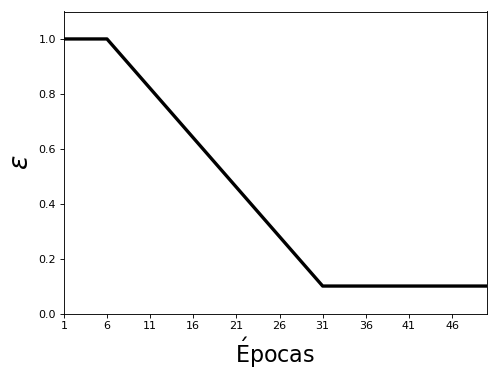
\includegraphics[width=200pt]{epsilon-decay.png}
                    \caption{\todo{fazer o grafico usando tikz} Fonte:}
                    \label{fig:epsilon-decay}
                \end{figure}
            \end{itemize}
        
\section{Função valor-ação}

    Função valor-ação ótima:

    \begin{equation}
        q_*(a) \ \dot{=} \ \mathbb{E}[R_t \mid A_t = a]
    \end{equation}

    Escolha gulosa:

    \begin{equation}
        A_t \ \dot{=} \ \argmax_a Q_t(a)
    \end{equation}
    
    \begin{center}
    \begin{tikzpicture}[->,>=stealth', auto, node distance=4.0cm, thick]
        \node[state-node]  (S1) {$s_1$};
        \node[state-node]  (S2) [below of=S1, xshift=-3.0cm] {$s_2$};
        \node[state-node]  (S3) [below of=S1, xshift= 3.0cm] {$s_3$};
        \node[hidden-node] (A1) [above of=S2, yshift=-1.5cm] {};
        \node[hidden-node] (A2) [below of=S1, yshift=2.5cm]  {};
        
        \draw[bend right=20,-] (S1) to node[action-label]           {$a_1$} (A1);
        \draw[-]               (S1) to node[action-label, pos=0.4]  {$a_2$} (A2);
        \draw[bend left=40]    (S1) to node[action-label, pos=0.25] {$a_3$} (S3);
        
        \draw[bend right=30]   (A1) to node[left, pos=0.2]  {$p_1$} (S2);
        \draw[bend left=30]    (A1) to node[right, pos=0.2] {$p_2$} (S2);
        \draw[bend left=40]    (A2) to node[left, pos=0.3]  {$p_3$} (S2);
        \draw[bend right=40]   (A2) to node[right, pos=0.3] {$p_4$} (S3);
        
        \draw[hidden-edge, bend right=30] (A1) to node[reward-label]           {$r_1$} (S2);
        \draw[hidden-edge, bend left=30]  (A1) to node[reward-label]           {$r_2$} (S2);
        \draw[hidden-edge, bend left=40]  (A2) to node[reward-label]           {$r_3$} (S2);
        \draw[hidden-edge, bend right=40] (A2) to node[reward-label]           {$r_4$} (S3);
        \draw[hidden-edge, bend left=40]  (S1) to node[reward-label, pos=0.65] {$r_5$} (S3);
    \end{tikzpicture}
    \end{center}
    
    Para simplificar o grafo, na maioria das vezes os nós das ações serão omitidos e as ações serão indicadas nos rótulos das arestas. Além disso, se a probabilidade for 1, ela é omitida.
    
    \subsection{Definição}
    
    \subsection{Versão incremental}
        
        \begin{equation}
            Q_n \ \dot{=} \ \frac{R_1 + R_2 + \cdots + R_{n-1}}{n - 1}
        \end{equation}
        
        \begin{equation}
        \begin{split}
            Q_{n+1} & \ \dot{=} \ \frac{1}{n} \sum_{i=1}^{n} R_i \\
            & = \ Q_n + \frac{1}{n} \Big[ R_n - Q_n \Big]
        \end{split}
        \end{equation}
        
        Ver no livro a derivação dessa equação (eq. 2.3).
        
        \begin{equation}
            NovaEstimativa \leftarrow AntigaEstimativa + TamanhoPasso \Big[ Objetivo - AntigaEstimativa \Big]
        \end{equation}
        
        \begin{equation}
        \begin{split}
            Q_{n+1} & \ \dot{=} \ Q_n + \alpha \Big[ R_n - Q_n \Big] \\
            & = \ (1 - \alpha)^n Q_1 + \sum_{i=1}^{n} \alpha (1 - \alpha)^{n - i} R_i
        \end{split}
        \end{equation}
        
    \subsection{Escolha dos valores iniciais}
        
        Obs.: citar a diferença entre problemas estacionários e não-estacionários
        
        \subsubsection{Valores otimistas}
        
        \subsubsection{Limite Superior de Confiança (UCB)}
        
\section{Tarefas \todo{ou problema?, verificar texto todo} Não-Associativas, Associativas e o Problema Completo do Aprendizado por Reforço}

    \subsection{Nonassociative}
    
        Um problema \emph{não-associativo} é basicamente um problema em que não uma mudança de ambiente \todo{configuração seria melhor? verificar no sutton}. Assim, após uma ação ser escolhida, o agente recebe a recompensa adequada e volta para o início do problema. 
        
        \begin{center}
            \simplebandit
        \end{center}
        
        Para resolver um problema não-associativo utilizamos as técnicas de avaliação das ações discutidas anteriormente.

    \subsection{Associative}
    
        Em um problema \emph{associativo} o ambiente pode mudar após uma ação ser escolhida. Nesse caso, existem diversas configurações de ambientes diferentes e uma delas será aquela a ser avaliada no momento. Observe que a escolha de uma ação não influencia na configuração encontrada na iteração seguinte.

        \begin{center}
            \associativebandits
        \end{center}
        
        Para resolver esse tipo de problema não podemos utilizar as técnicas de avaliação da função de valor da ação, pois o ambiente pode mudar completamente na iteração seguinte. Dessa forma, é necessário que haja uma informação adicional sobre qual ambiente está sendo jogado agora, para que possamos fazer um mapeamento de cada um deles, assim podemos ter uma resposta ótima para cada. Esse tipo de mapeamento se chama \emph{política} e será explorado no futuro.
        
    \subsection{Full RL Problem}
    
        O \emph{problema completo de aprendizado por reforço} é um passo além de um não-associativo, pois cada ação levará a um determinado ``ambiente''. 
    
        \begin{center}
            \fullrldiagram
        \end{center}
        
        Nesse caso, não precisamos de uma informação adicional sobre o ambiente/estado em que estamos, já que essa informação pode ser encontrada diretamente a partir dos pares (estado, ação). Mas ainda é necessário mapear as melhores ações a partir de cada estado e para isso utilizaremos uma \emph{política}. É justamente sobre o problema completo do aprendizado por reforço que trataremos a seguir. Mais especificamente sobre sua formalização como um \emph{Processo de Decisão de Markov}.
        
    \subsection{Problema estacionário}

        Por exemplo, um simples problema não-estacionário pode ser visto nos diagramas abaixo. Note que $p_1 \neq p_2$ e $q_1 \neq q_2$, caso contrário seria um problema estacionário. 

        \begin{figure}[h]
            \centering
            \begin{subfigure}{.3\linewidth}
                \centering
                \begin{tikzpicture}[-,>=stealth', auto, node distance=1.5cm, thick]
                    \node[state-node]  (S1) {$s$};
                    \node[reward-node] (R1) [below of=S1, xshift=-1.0cm] {$r$};
                    \node[reward-node] (R2) [below of=S1, xshift=1.0cm]  {$r$};
                    
                    \draw[bend right] (S1) to node[left, pos=0.8] {$p_1$} (R1);
                    \draw[bend left]  (S1) to node[right, pos=0.8] {$q_1$} (R2);
                    
                    \draw[hidden-edge, bend right] (S1) to node[action-label] {$a_1$} (R1);
                    \draw[hidden-edge, bend left]  (S1) to node[action-label] {$a_2$} (R2);
                \end{tikzpicture}
                \caption{Momento 1}
            \end{subfigure}
            \begin{subfigure}{.3\linewidth}
                \centering
                \begin{tikzpicture}[-,>=stealth', auto, node distance=1.5cm, thick]
                    \node[state-node]  (S1) {$s$};
                    \node[reward-node] (R1) [below of=S1, xshift=-1.0cm] {$r$};
                    \node[reward-node] (R2) [below of=S1, xshift=1.0cm]  {$r$};
                    
                    \draw[bend right] (S1) to node[left, pos=0.8] {$p_2$} (R1);
                    \draw[bend left]  (S1) to node[right, pos=0.8] {$q_2$} (R2);
                    
                    \draw[hidden-edge, bend right] (S1) to node[action-label] {$a_1$} (R1);
                    \draw[hidden-edge, bend left]  (S1) to node[action-label] {$a_2$} (R2);
                \end{tikzpicture}
                \caption{Momento 2}
            \end{subfigure}
            \caption{Teste}
        \end{figure}
        
\section{Recompensas imediatas e tardias}

    ... é chamado de \emph{distribuição de recompensas}

    \subsection{Recompensas imediatas}
    
        \begin{center}
        \begin{tikzpicture}[-,>=stealth', auto, node distance=2.0cm, thick]
            \node[state-node]  (S1) {$s_1$};
            \node[hidden-node] (H1) [above right of=S1] {};
            \node[state-node]  (S2) [below right of=H1] {$s_2$};
            \node[hidden-node] (H2) [above right of=S2] {};
            \node[state-node]  (S3) [below right of=H2] {$s_3$};
            \node[hidden-node] (H3) [above right of=S3] {};
            \node[state-node]  (S4) [below right of=H3] {$s_4$};
            \node[]            (HN) [above right of=S4] {$\cdots$};
            \node[state-node]  (SN) [below right of=HN] {$s_n$};
            \node[]            (SH) [below of=HN, yshift=0.5cm] {$\cdots$};
            
            \draw[-, bend left, out=30, in=140]  (S1) to node[action-label, pos=0.6] {$a_1$} (H1);
            \draw[->, bend left, out=40, in=150] (H1) to node[reward-label, pos=0.4] {$r_2$} (S2);
            \draw[-, bend left, out=30, in=140]  (S2) to node[action-label, pos=0.6] {$a_2$} (H2);
            \draw[->, bend left, out=40, in=150] (H2) to node[reward-label, pos=0.4] {$r_3$} (S3);
            \draw[-, bend left, out=30, in=140]  (S3) to node[action-label, pos=0.6] {$a_3$} (H3);
            \draw[->, bend left, out=40, in=150] (H3) to node[reward-label, pos=0.4] {$r_4$} (S4);
            \draw[-, bend left, out=30, in=135]  (S4) to node[action-label] {$a_4$} (HN);
            \draw[->, bend left, out=45, in=150] (HN) to node[reward-label] {$r_n$} (SN);
        \end{tikzpicture}
        \end{center}
        
        \begin{center}
            $s_1,\ a_1,\ \mathbf{r_2},\ s_2,\ a_2,\ \mathbf{r_3},\ s_3,\ a_3,\ \mathbf{r_4},\ s_4,\ a_4,\ \dots\,\ \mathbf{r_n},\ s_n$
        \end{center}
        
        temos um total de n recompensas, o que caracteriza um \todo{alguma coisa} de recompensas \emph{densas}.
    
    
    \subsection{Recompensas tardias}
    
        \begin{center}
        \begin{tikzpicture}[-,>=stealth', auto, node distance=1.5cm, thick]
            \node[state-node]  (S1) {$s_1$};
            \node[hidden-node] (H1) [above right of=S1] {};
            \node[state-node]  (S2) [below right of=H1] {$s_2$};
            \node[hidden-node] (H2) [above right of=S2] {};
            \node[state-node]  (S3) [below right of=H2] {$s_3$};
            \node[hidden-node] (H3) [above right of=S3] {};
            \node[state-node]  (S4) [below right of=H3] {$s_4$};
            \node[]            (HN) [above right of=S4, xshift=0.5cm, yshift=0.3cm] {$\cdots$};
            \node[state-node]  (SN) [below right of=HN, xshift=0.5cm, yshift=-0.3cm] {$s_n$};
            \node[]            (SH) [below of=HN] {$\cdots$};
            
            \draw[->, bend left, out=40, in=150] (H1) to node {} (S2);
            \draw[->, bend left, out=40, in=150] (H2) to node {} (S3);
            \draw[->, bend left, out=40, in=150] (H3) to node {} (S4);
            \draw[->, bend left, out=45, in=150] (HN) to node[reward-label] {$r_n$} (SN);
            
            \draw[-, bend left, out=30, in=140]  (S1) to node[action-label, pos=1.0] {$a_1$} (H1);
            \draw[-, bend left, out=30, in=140]  (S2) to node[action-label, pos=1.0] {$a_2$} (H2);
            \draw[-, bend left, out=30, in=140]  (S3) to node[action-label, pos=1.0] {$a_3$} (H3);
            \draw[-, bend left, out=30, in=135]  (S4) to node[action-label] {$a_4$} (HN);
        \end{tikzpicture}
        \end{center}
        
        \begin{center}
            $s_1,\ a_1,\ s_2,\ a_2,\ s_3,\ a_3,\ s_4,\ a_4,\ \dots\,\ \mathbf{r_n},\ s_n$
        \end{center}
        
        Temos somente uma única recompensa ao fim do episódio, o que caracteriza um \todo{alguma coisa, olhar no sutton} de recompensas \emph{esparsas}.
        
\end{document}
